\chapter{Conclusions}

This chapter presents the general remarks about the work done in this dissertation while introducing some possible improvements for future work.

\section{Discussion}

The objectives defined in the first chapter for this thesis were fully achieved. However, like last year, the end results are not satisfactory .


Given the complexity and difficulty of creating a fully automatic image retrieval system and considering the limitation in research in this area and the extreme amount of computing processing time and resources a system of this kind requires, it can be concluded that the results of this work open the possibility for more exploration into to the development of a more robust system.


With the current state-of-the-art and computer technology fully automatic retrieval systems cannot surpass interactive systems in performance. Some very good reasons for this is that interactive systems offer user visualization, user interaction and user decision. This helps the system to be tremendously more accurate than a computer, since the user can correct the computer if the retrieved images are not related to the topic.


However even though the end results have low-score it was still possible to present results that prove that the automatic retrieval system built was capable, in some situations, of working like intended. This was shown in the given example in chapter \ref{ch:results} section \ref{sec:run1} where the pictures returned in the first run did indeed belong to the moment that was described in the test topic. This concludes that a system like this can work, and can contribute to the improvement of the quality of life of the human kind, however it still requires a lot of improvement.



\subsection{System Strengths}

\begin{itemize}
    \itemsep0em
    \item Capable of fully processing a big dataset of images, extracting dates, object labels and scene labels.
    \item The system is modular, which means it can be easily added new algorithms to fine-tune the image processing or more linguistic rules that can achieve better text mining results.
    \item Capable of text processing and word extraction to specific predefined categories.
    \item Capable of self-evaluation using the F1-measure@xx if the ground truth is available.
\end{itemize}


\subsection{System Weaknesses}

\begin{itemize}
    \itemsep0em
    \item Requires a lot of processing time in order to retrieve images of a big dataset.
    \item Requires good computer specs.
    \item Low-score end results.
\end{itemize}

\section{Future Work}

A few things can be done in order to improve system performance for the 2021 imageclef LMRT sub-task.

Firstly the text processing and word extraction stage can be improved in order to only extract meaningful words. Sometimes in the extractions, words that had no meaningful use and were only clutter were extracted. For example "evening time" was in the category "locations". In most cases this wont influence the score much, but will increase processing time. This is because "evening time" will be compared with all of the images extracted "locations" from the organizers data. Another aspect that needs improving is the extraction of negative words which is very dependent on how the sentence is worded.

Using more powerful computers and optimize the system is essential in order to conduct a more large quantity of tests and fine tune the system. Currently the system is so slow, that the fine-tuning process becomes complex.

Since most of the dataset is comprised of folders of images of one full day, it could be possible to link a set of images like a video and implement activity video recognition algorithms in order to extract the activity of the images instead of using the organizers data, which was in most cases inaccurate. Furthermore, better scene recognition and even color recognition algorithms will definitely improve the f1-measure@10 scores. Also using algorithms to remove blurred images can help with the time it takes for the system to process the dataset.

Another future improvement would be to use the google cloud vision api, which gives labels that are more related to the words extracted. Some examples are given below.


\begin{figure}[H]
    \centering
    \captionsetup{justification=centering}
    \begin{subfigure}{0.45\textwidth}
    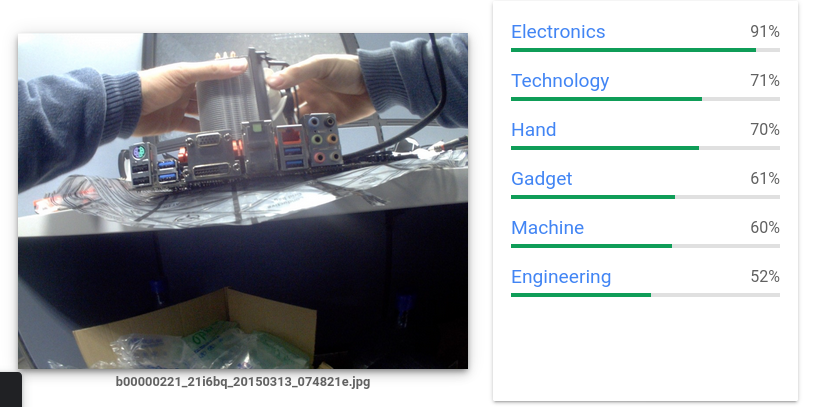
\includegraphics[width=\textwidth]{Sections/8Conclusion/images/google.png} 
  
    \end{subfigure}
    \begin{subfigure}{0.45\textwidth}
    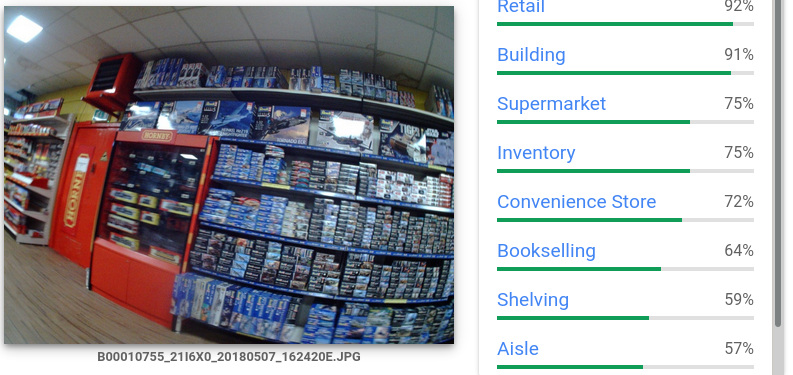
\includegraphics[width=\textwidth]{Sections/8Conclusion/images/labels.png}
    \end{subfigure}

  \end{figure}


\begin{figure}[H]
    \centering
    \captionsetup{justification=centering}

    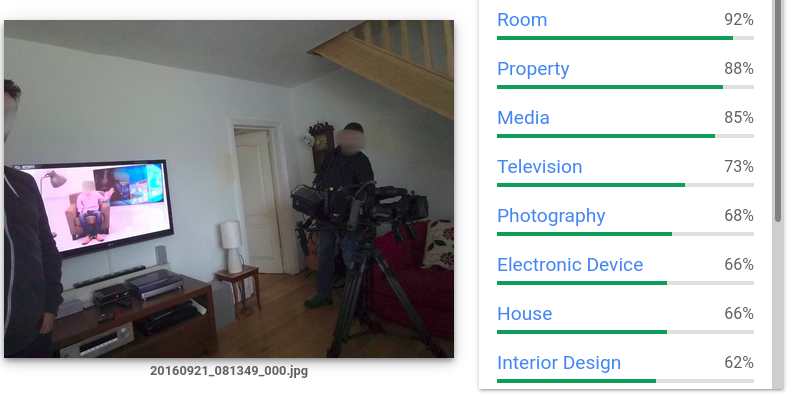
\includegraphics[width=0.45\textwidth]{Sections/8Conclusion/images/google_labels_2.png}
    
    \caption{Examples of google API extracted labels .}
\end{figure}
